\documentclass[11pt]{article}
\newcommand\tab[1][1cm]{\hspace*{#1}}
\usepackage{graphicx}
\usepackage{float}

\begin{document}
	\title{Ticket Salad Admin Portal User Manual}
	\date{Hackermen}
		
	\author{Tristan Joseph \\ Jarryd Baillie \\ Brandon Teixeira \\ Gift Mothusi \\ Thomas Honiball }

		
	\maketitle
	\tableofcontents
	\newpage
	
	\section{System Overview}
	The Ticket Salad Admin Portal is a web-based management system for the mobile application. This portal allows administrators to add, delete and update any events that will reflect on the Ticket Salad mobile application.
	
	\section{System Configuration}
	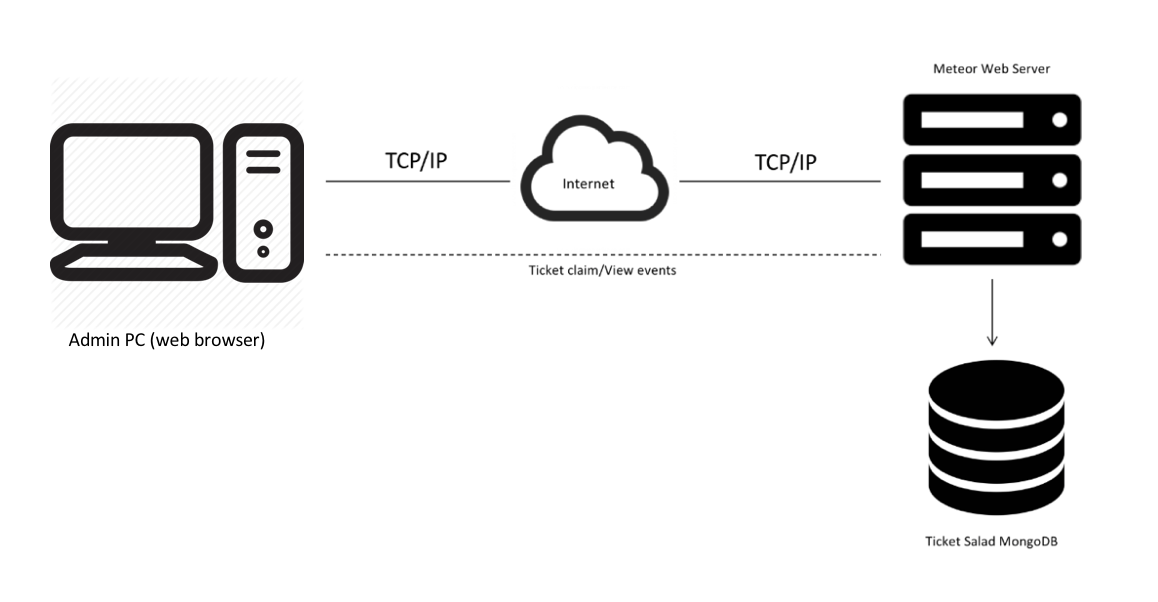
\includegraphics[width=\linewidth]{diagram.png}
	\section{Installation}
	
	Since the Admin Portal is web-based, no installation is required and is simply accessed through any web browser.
	
	\section{Getting Started}
	An admin must have an admin username and password to gain access to the portal, once accessed the admin will see a list of all current live events on the Ticket Salad system. A search bar is located at the top left to filter through events. An admin may add a new event or edit/delete an existing event. The admin can also sign out of the portal by clicking on their name at the top right of the screen and clicking "sign out".
	\\
	\pagebreak

	\section{Using the system}
	\subsection{Logging In}
	Once the admin has the valid credentials to use the portal, the username and password may be entered in the respective fields in order to gain access to the portal's main page.
	\\
	\\
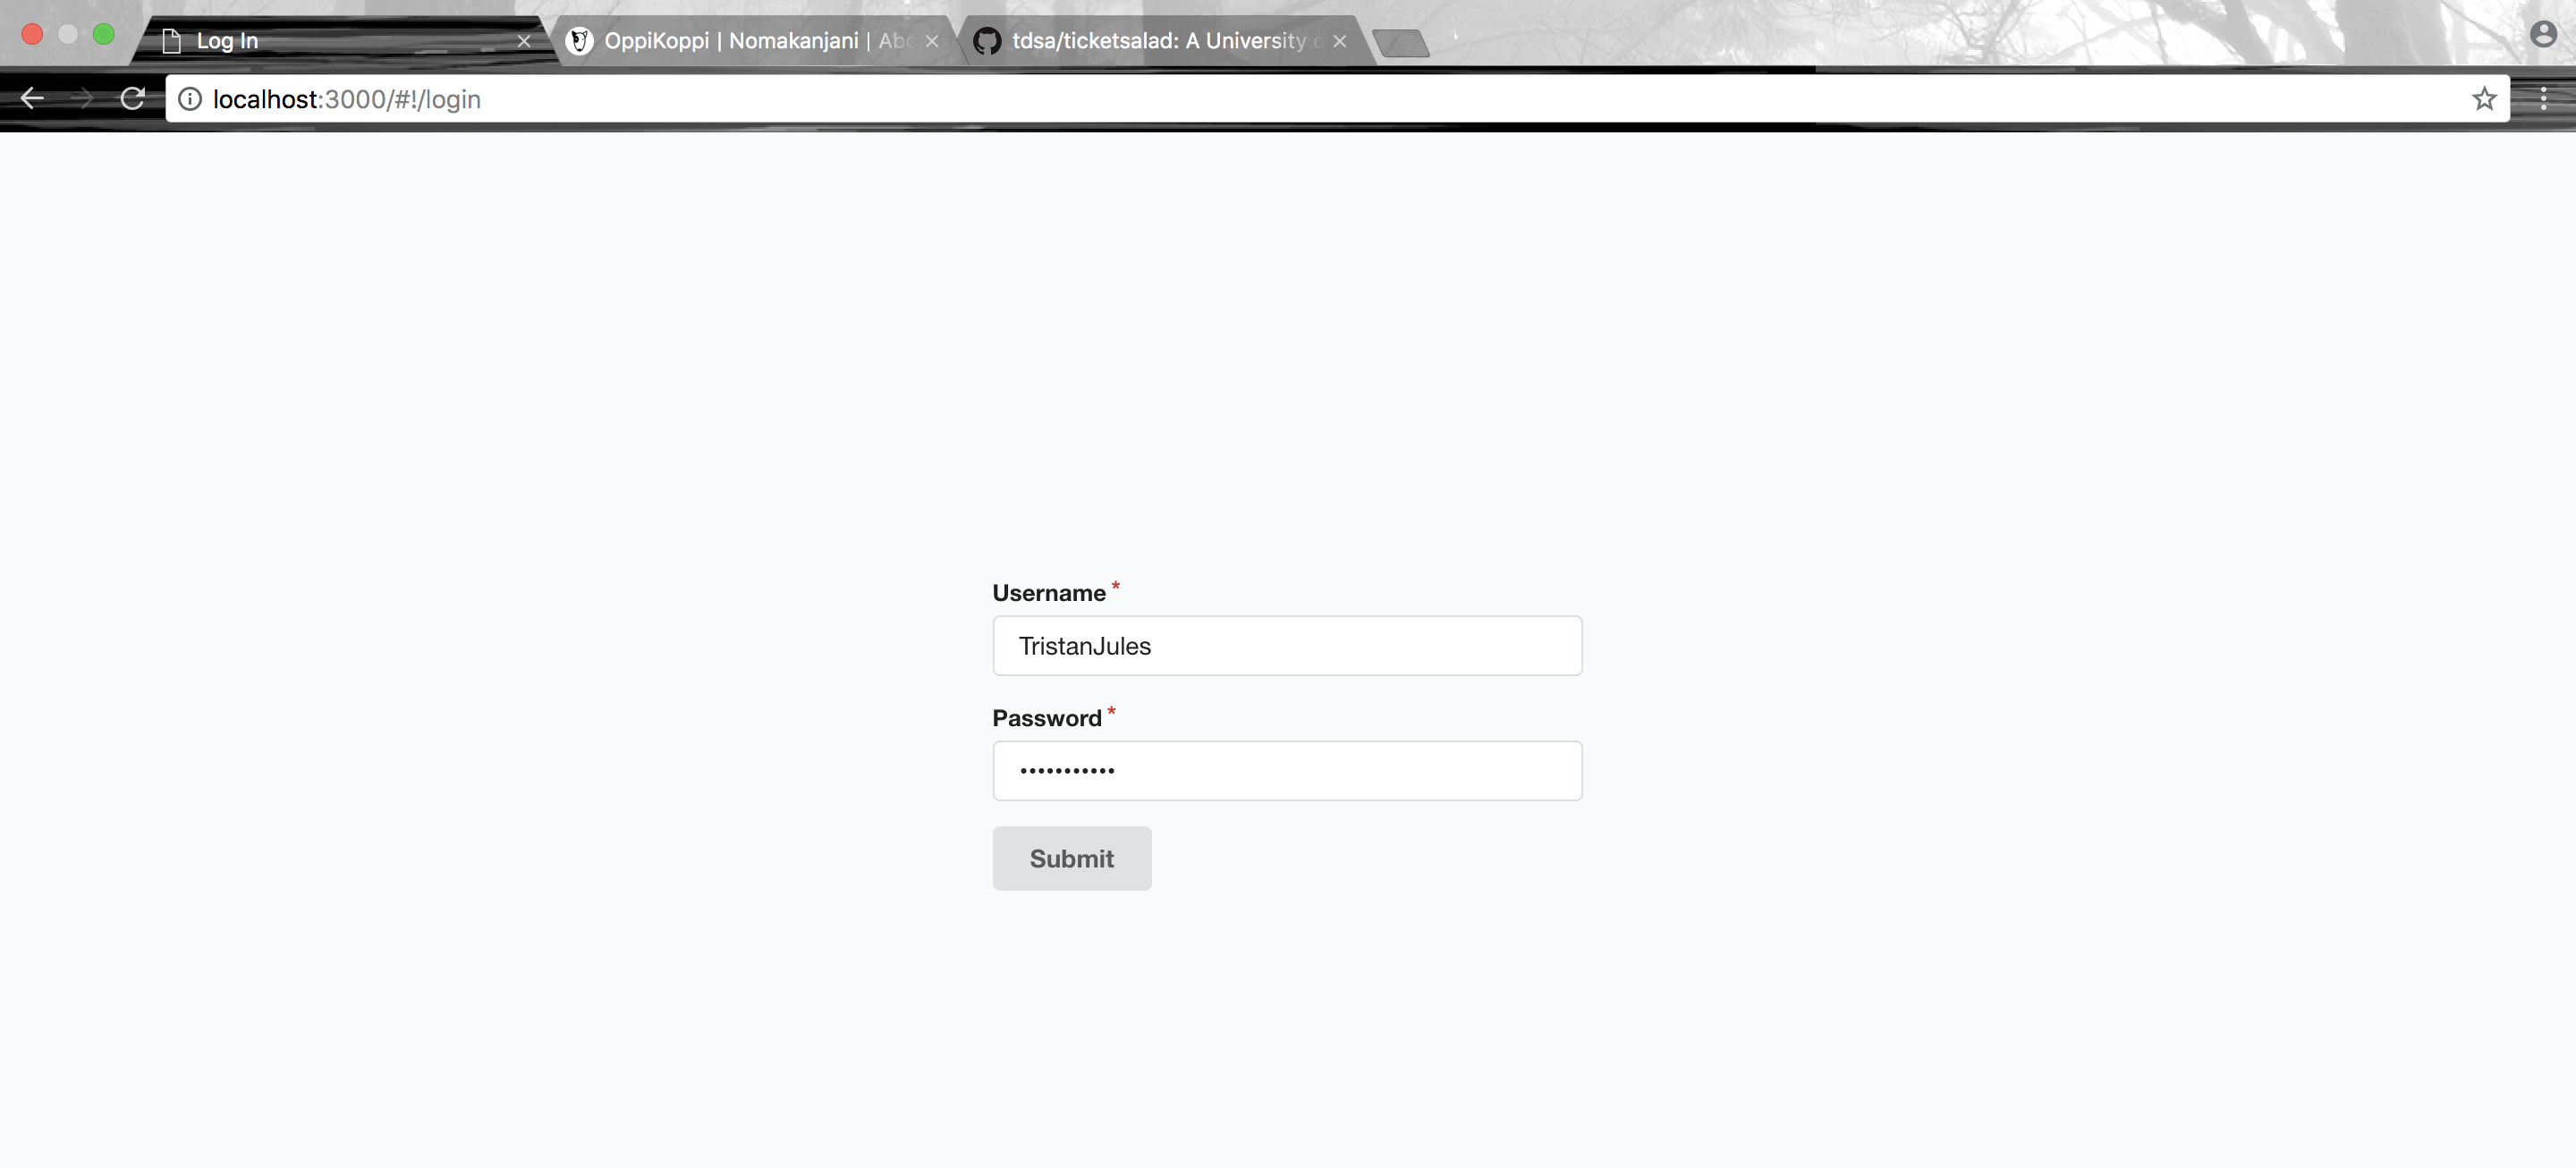
\includegraphics[width=\linewidth]{login.png}
\pagebreak
	\subsection{Event Listing}
	Once the admin has logged in, a page will be displayed listing all current live events. From this page an admin may edit or delete any event as well as add a new event (shown in the top right corner of the screen). The admin may also sign out from this page.
	\\
	\\
	
\includegraphics[width=\linewidth]{home.png}
	\pagebreak
	\subsection{Adding an Event}
	The admin must specify all details relating to an event when clicking the "add event" button before submitting. Once submitted, the event will immediately be accessible from all platforms.
	\\
	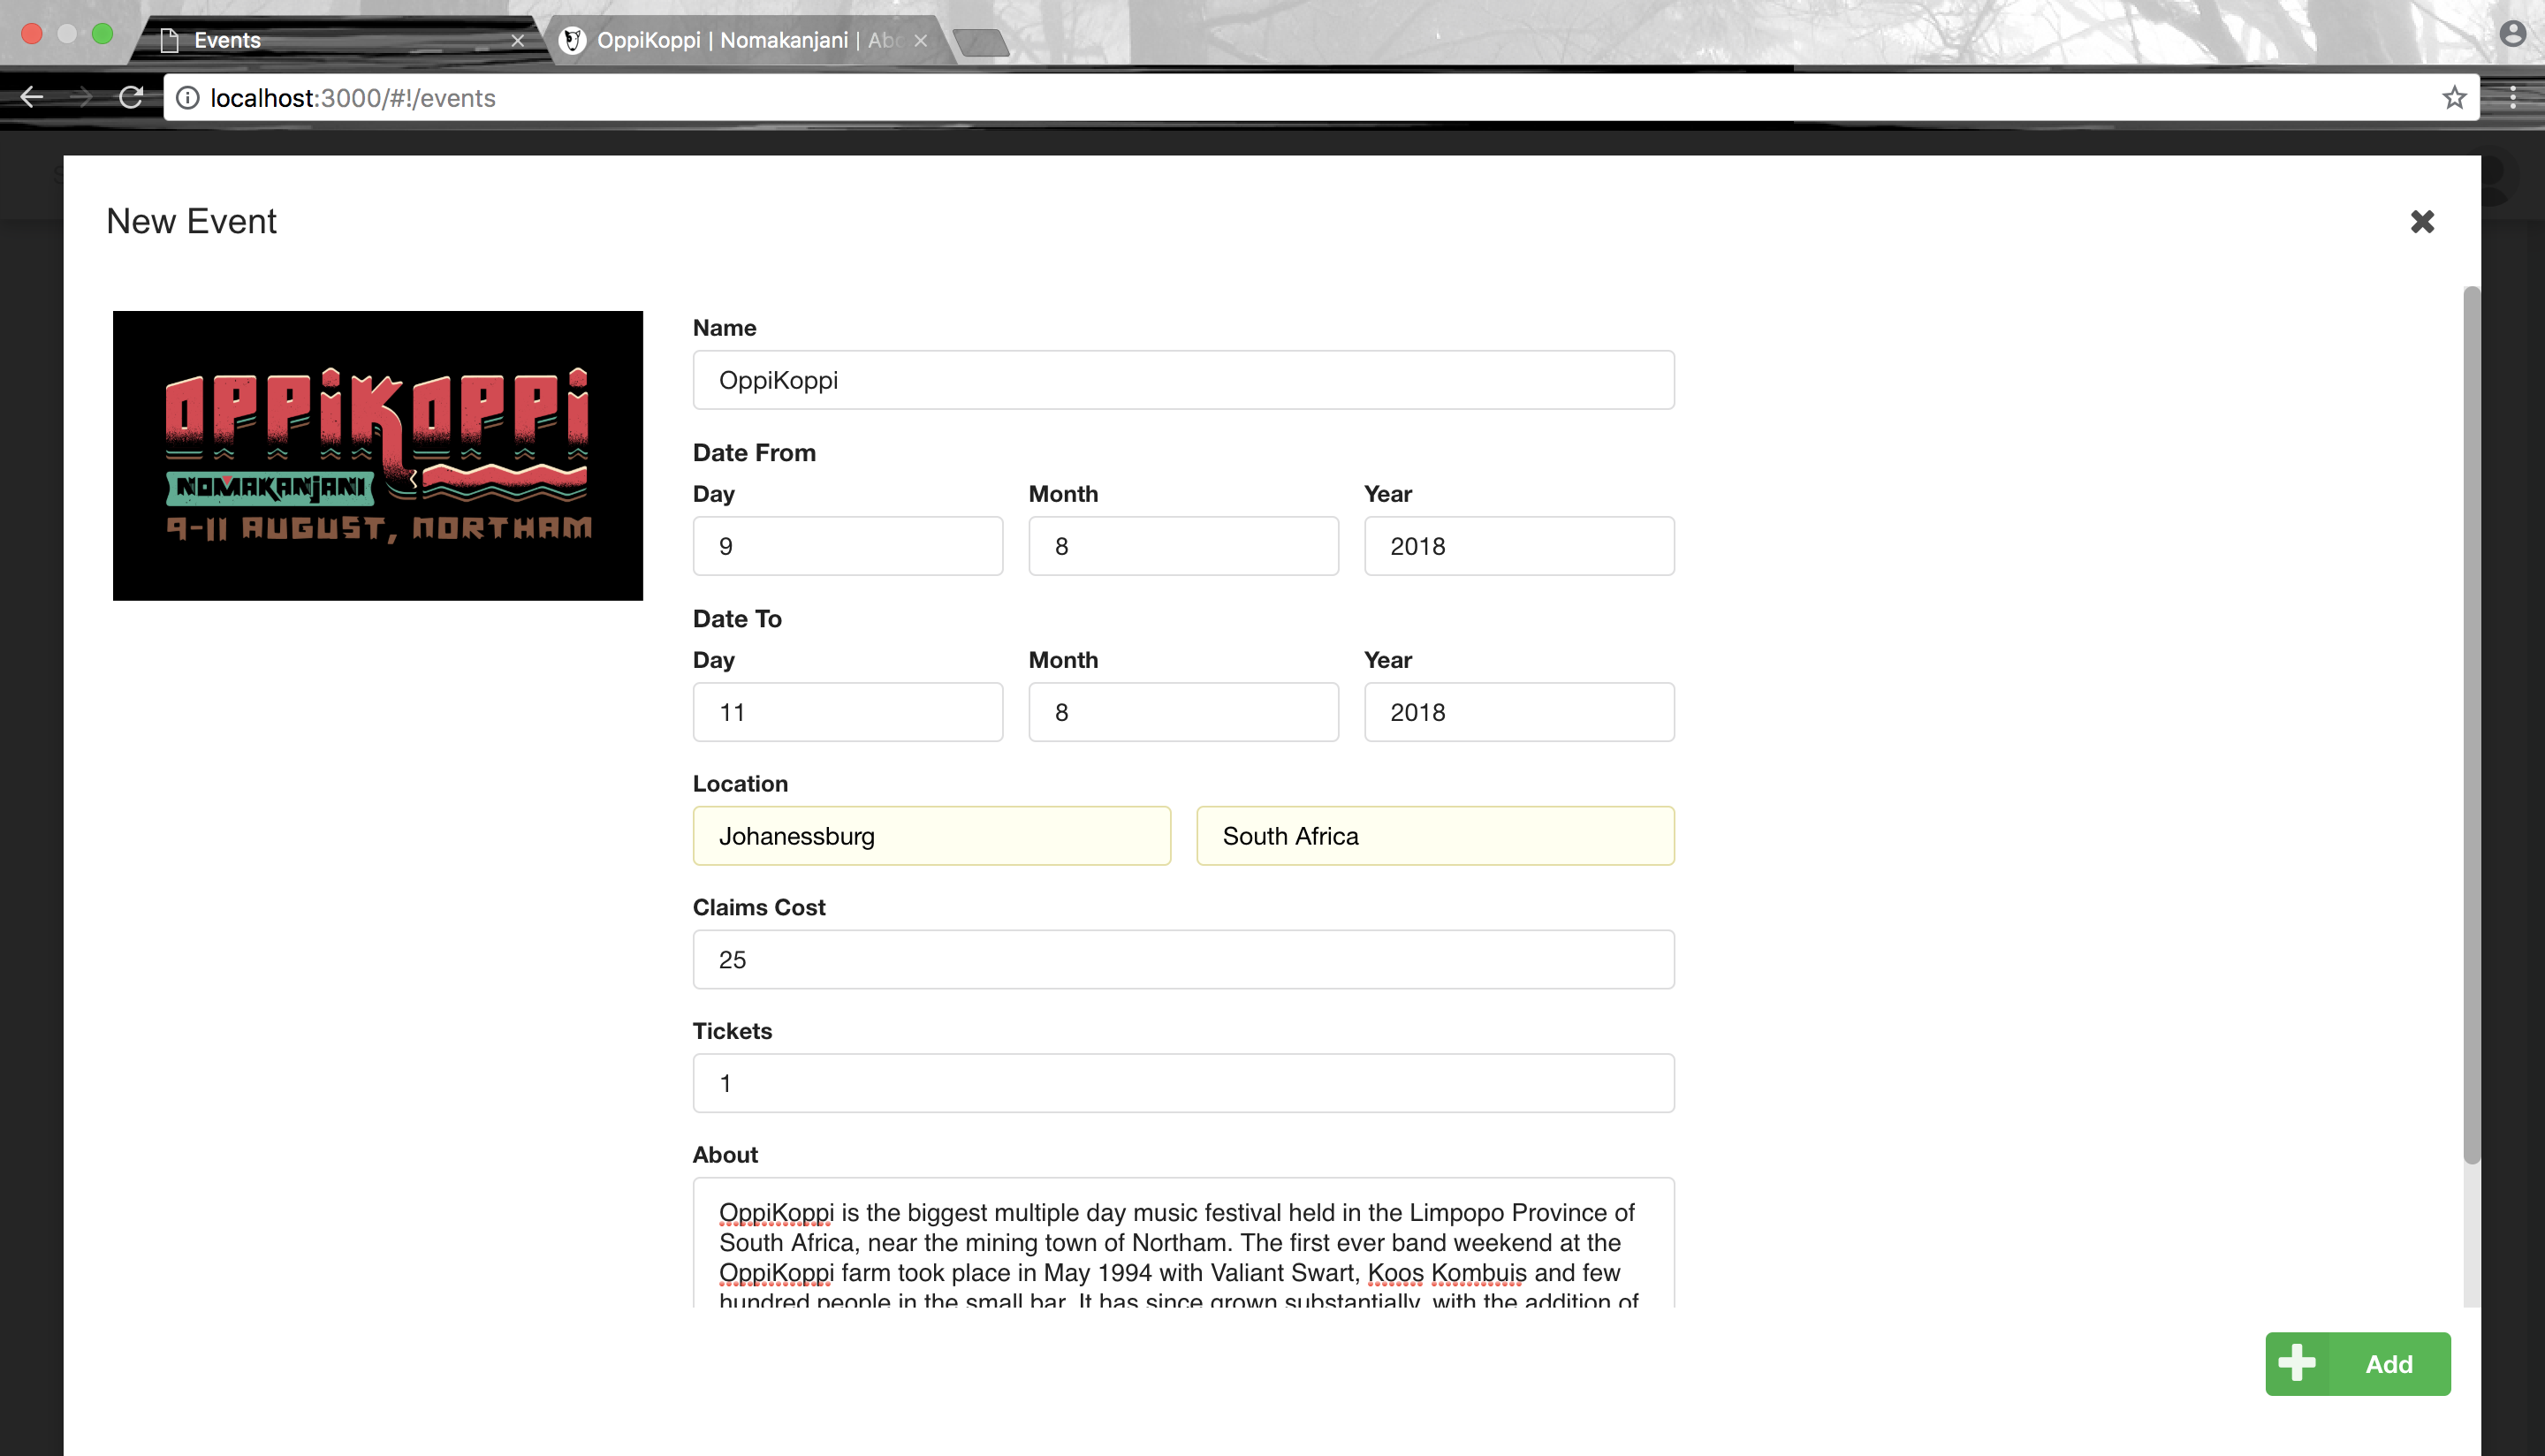
\includegraphics[width=\linewidth]{add.png}

	\pagebreak
	\subsection{Editing an event}
	Events are editable in order to make corrections and/or updates to events. Any field can be edited and similarly to the "Add Event" option, all fields must be valid in order to submit changes. All changes will reflect immediately across all platforms.
	\\

	\subsection{Deleting an Event}
	All events can easily be deleted by clicking on the event and clicking the "Delete" button. The admin will be prompted to continue as deleting an event cannot be reversed. 
	\\
	\\

	\section{Troubleshooting}
	\subsection{Invalid Login Details}
	If an admin is being denied access to the portal through the login system, it is most likely due to an incorrect
	email and password combination. This must be retrieved by a system administrator as there is no forgot password option.
	\subsection{Server Downtime}
	In the event that server maintenance is required, possible server downtime will occur leaving all Ticket Salad 
	services offline. This downtime will be temporary and user's will be notified beforehand.
	\subsection{Invalid Details}
	When Adding or editing an event, it is important all values entered in each field are valid and correct, the system will not accept data that is invalid (such as a string for a date).
	
\end{document}




















